% ============================================================
%  附录E 泊松求和公式
%  底本：高等教育出版社《固体理论》第二版；原书印刷页 552–553
%  （PDF 页 = 印刷页 + 20）
%  公式编号自检：(E.1)–(E.10)，自动编号 10 个，无缺号。
%
%  已修正的 OCR/原书错误（除全角句点转"."、删 ~ 间隔符、收紧
%  \mathrm{d}、拆开行内公式与中文等常规项外）：
%  1. (E.2) 括注 OCR 乱码"( n Σ*Σ )"按 p552 复原为"(n 为整数)"。
%  2. (E.5) 两处 lim 下标 OCR 丢箭头，按 p552 补"z→iω_n"。
%  3. 正文"[−βf(z)]"两处 OCR 乱码（\mathbf{\Lambda} 等）按
%     p552 复原。
%  4. 图 E.1 图例两行 OCR 乱码按 p552 复原为
%     ""×"——f(z)的极点，""·"——(z−x)^{-1}的极点"。
%  5. (E.7) 前文"沿实轴的上岸从−∞→∞"OCR 丢箭头按 p553 补；
%     "只包含 z=x 处的极点"OCR 乱码按 p553 复原。
%  6. (E.9) 首行及其前文的函数"[tanh(1/2)βx]/x"OCR 误作 βα，
%     按 p553 复原为 βx。
%  7. (E.9) 后文"对正 n 值求和"OCR 衍出"$f$"（成"求 f 和"），
%     按 p553 删。
%  8. 章末句"临界磁场 H_c(T)"后按 p553 补句点。
%  插图：图 E.1 泊松求和公式的回路（原书印刷 p552/PDF p572），
%  占位图 figures/figE-1.pdf（由 MinerU 裁剪图转 PDF 生成），
%  图例两行随图排。
%  遗留问题：无
% ============================================================
\chapter{泊松求和公式}

费密分布函数的下列级数展开式称为泊松(Poisson)求和公式
\begin{equation}
  f(x)=\frac{1}{\mathrm{e}^{\beta x}+1}
  =\frac{1}{\beta}\sum_{n=-\infty}^{\infty}
  \frac{\mathrm{e}^{\mathrm{i}\omega_{n}\eta}}{\mathrm{i}\omega_{n}-x}
\end{equation}
其中 $\beta=(k_{\mathrm{B}}T)^{-1}$，$\eta=+0$，而
\begin{equation}
  \omega_{n}\equiv(2n+1)\pi k_{\mathrm{B}}T
  \qquad(\text{$n$ 为整数})
\end{equation}
式(E.1)是一个有用的计算公式，其证明如下：

由于
\begin{equation}
  \mathrm{e}^{\mathrm{i}\beta\omega_{n}}
  =\mathrm{e}^{\mathrm{i}(2n+1)\pi}=-1
\end{equation}
因此，在 $z$ 复平面中费密函数可写成
\begin{equation}
  f(z)=\frac{1}{\mathrm{e}^{\beta z}+1}
  =\frac{1}{1-\mathrm{e}^{\beta(z-\mathrm{i}\omega_{n})}}
\end{equation}
它在虚轴上 $z=\mathrm{i}\omega_{n}$ 有奇点，这些奇点对称分布在实轴上下，如图E.1中“$\times$”号点所示.不难证实，$[-\beta f(z)]$ 函数有一组留数为1的极点，因为
\begin{equation}
  \lim_{z\to\mathrm{i}\omega_{n}}(z-\mathrm{i}\omega_{n})
  \left[-\beta f(z)\right]
  =\lim_{z\to\mathrm{i}\omega_{n}}
  \frac{(-\beta)(z-\mathrm{i}\omega_{n})}
  {1-\mathrm{e}^{\beta(z-\mathrm{i}\omega_{n})}}=1
\end{equation}
这时沿回路 $C$ 的下列积分可以用 $[-\beta f(z)]$ 的留数表示，得到等式
\begin{equation}
  \frac{1}{2\pi\mathrm{i}}\int_{C}\mathrm{d}z
  \frac{f(z)\mathrm{e}^{z\eta}}{z-x}
  =-\frac{1}{\beta}\sum_{n=-\infty}^{\infty}
  \frac{\mathrm{e}^{\mathrm{i}\omega_{n}\eta}}{\mathrm{i}\omega_{n}-x}
\end{equation}
由于公式(E.6)左边被积函数 $\left[f(z)\mathrm{e}^{z\eta}/(z-x)\right]$ 在 $z$ 复平面中（除实轴和虚轴以外的地方）是解析函数，因此利用约当(Jordan)引理可将沿回路 $C$ 的积分换为沿 $\Gamma+C'$ 回路的积分，这里 $\Gamma$ 是半径趋向无穷大的圆弧.考虑到 $\mathrm{e}^{z\eta}$ 因子的存在，当 $\mathrm{Re}\,z<0$ 时沿左半复平面 $\Gamma$ 上的被积函数将指数式趋向零.对于 $\mathrm{Re}\,z>0$ 情况，被积函数中的 $f(z)$ 将提供 $\mathrm{e}^{-\beta z}$ 因子，同样使得沿右半复平面的 $\Gamma$ 积分为零.

\begin{center}
\begin{minipage}{6.5cm}
\centering
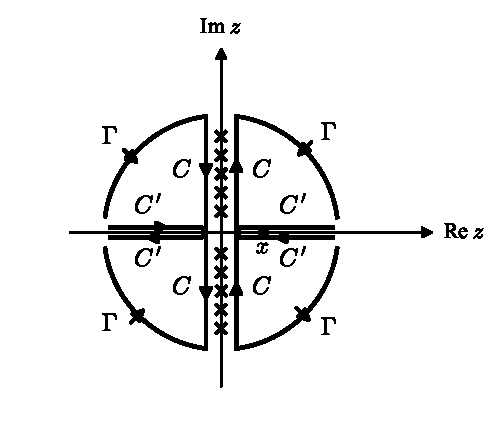
\includegraphics[width=6.5cm]{figE-1.pdf}\\*[0.3em]
{\small “$\times$”——$f(z)$的极点，}\\*[0.2em]
{\small “$\cdot$”——$(z-x)^{-1}$的极点}\\*[0.2em]
{\small 图 E.1\quad 泊松求和公式的回路}
\end{minipage}
\end{center}

这样可求出关系式
\begin{equation}
  \frac{1}{2\pi\mathrm{i}}\int_{C}\mathrm{d}z
  \frac{f(z)\mathrm{e}^{z\eta}}{z-x}
  =\frac{1}{2\pi\mathrm{i}}\int_{C'}\mathrm{d}z
  \frac{f(z)\mathrm{e}^{z\eta}}{z-x}
\end{equation}
式(E.7)相当于把绕虚轴的回路 $C$ 扭曲为 $C'$ 回路，使积分沿实轴的上岸从 $-\infty\to\infty$，然后再从实轴的下岸回到 $-\infty$ 处，由于沿 $C'$ 回路只包含 $z=x$ 处的极点，因此
\begin{equation}
  f(x)=-\frac{1}{2\pi\mathrm{i}}\int_{C'}\mathrm{d}z
  \frac{f(z)\mathrm{e}^{z\eta}}{z-x}
\end{equation}
再利用式(E.6)和(E.7)，即得泊松求和公式(E.1).

利用泊松求和公式可将函数 $\left[\tanh\frac{1}{2}\beta x\right]/x$ 表示为
\begin{equation}
\begin{aligned}
  \frac{\tanh\frac{1}{2}\beta x}{x}
  &=\frac{f(-x)-f(x)}{x}\\
  &=\frac{1}{\beta}\sum_{n=-\infty}^{\infty}
  \mathrm{e}^{\mathrm{i}\omega_{n}\eta}\frac{1}{x}
  \left[\frac{1}{\mathrm{i}\omega_{n}+x}
  -\frac{1}{\mathrm{i}\omega_{n}-x}\right]\\
  &=\frac{2}{\beta}\sum_{n=-\infty}^{\infty}
  \frac{\mathrm{e}^{\mathrm{i}\omega_{n}\eta}}
  {\omega_{n}^{2}+x^{2}}
\end{aligned}
\end{equation}
由于 $f$ 函数的极点对称分布于实轴上下，式(E.9)可简化为对正 $n$ 值求和，再考虑到 $\eta=+0$，从式(E.9)求出下列有用公式
\begin{equation}
  \frac{\tanh\frac{1}{2}\beta x}{x}
  =\frac{4}{\beta}\sum_{n=0}^{\infty}
  \frac{1}{\omega_{n}^{2}+x^{2}}
\end{equation}
上式在超导理论中用于计算 $T\to T_{\mathrm{c}}$ 时的能隙 $\Delta(T)$ 和临界磁场 $H_{\mathrm{c}}(T)$.
